\subsection{Методы доступа к среде}
\label{sec:methods}

Дополнение IEEE 802.11e~\cite{802.11e} к стандарту Wi-Fi, направленное на внедрение поддержки QoS-требований, определило два новых механизма доступа: EDCA (Enhanced Distributed Channel Access) и HCCA (Hybrid coordination function Controlled Channel Access). Первый из них является механизмом приоритезированного случайного доступа к каналу, а второй --- механизмом детерминированного доступа.

С ростом плотности Wi-Fi-сетей HCCA и EDCA оказались не способны обеспечить надежную передачу данных, так как не обладают возможностями по работе в условиях жесткой интерференции. В частности, в случае большого числа точек доступа, работающих в одной области пространства, многие точки доступа выбирают один и тот же частотный канал. В результате EDCA страдает от множественных коллизий и эффекта скрытых станций. Ситуация с HCCA лишь немногим лучше за счет того, что HCCA исключает интерференцию со станциями своей сети. Поэтому возникает необходимость в разработке новых механизмов доступа, рассчитаных на работу в плотных сетях Wi-Fi.

Например, дополнение IEEE 802.11aa определяет механизм HCCA TXOP Negotiation, который позволяет точке доступа зарезервировать последовательность периодических интервалов времени, в течение которых она опрашивает свои станции, а соседние точки доступа (вместе со своими станциями) хранят молчание.  Данный подход существенно уменьшает интерференцию с соседними сетями, повышая надежность передачи. Стоит отметить, что интервалы времени резервируются не по одному, а целыми последовательностями: точка доступа резервирует \textit{последовательность периодических интервалов времени равной длительности}, в дальнейшем называемую \textit{периодическим резервированием}. Благодаря периодичности, все резервирование может быть описано с помощью всего лишь трех величин: \textit{периода} зерезервированных интервалов, их \textit{длительности} и \textit{момента начала первого интервала} (рис.~\ref{fig:periodic_reservation}).

\begin{figure}[h]
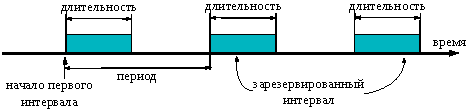
\includegraphics[width=\linewidth]{ReservedIntervals.pdf}
\caption{\label{fig:periodic_reservation} Периодическое резервирование}
\end{figure} 

Кроме дополнения IEEE 802.11aa периодические резервирования также присутствуют и в дополнении IEEE 802.11s (описывающим сети Wi-Fi Mesh). Это дополнение определяет механизм детерминированного доступа MCCA (Mesh coordination function Controlled Channel Access). MCCA позволяет любой станции в сети Wi-Fi Mesh установить периодическое резервирование, чтобы защитить собственные передачи от интерференции с соседними станциями. 

При использовании механизма комбинированного доступа для передачи мультимедийных данных реального времени с учетом QoS-требований, необходимо ответить на вопрос о том, как должны быть размещены зарезервированные интервалы времени, и когда станция должна использовать механизм случайного доступа. Первая попытка ответить на этот вопрос была сделана в дополнении  IEEE 802.11e, которое описывает механизм доступа, называемый HEMM (HCCA-EDCA Mixed Mode). Однако, в описании HEMM не указан способ выбора параметров, и только несколько работ  \cite{kuan2007utilization, lai2009adaptation, Ng2012, ruscelli2012enhancement} рассматривают использование этого механизма для передачи данных с QoS-требованиями.